\documentclass{article}
\usepackage[utf8]{inputenc}
\usepackage{graphicx}
\usepackage[spanish]{babel}


\begin{document}

\begin{figure}[t!]
\includegraphics[scale=0.3]{logo_udp.PNG}
\label{fig:udplogo}
\end{figure}

\title{\textbf{{Topología Física y Lógica \\ Redes de Datos \vspace{10cm}}}}
\author{\hspace{8cm} Vicente Henriquez \\ \hspace{8cm} Franco Montenegro}
\date{\hspace{8cm} 06/09/2017}
\maketitle

\newpage
\tableofcontents

\newpage
\section{Introducción \vspace{0.5cm}}
Una red puede definirse como un conjunto de nodos interconectados pero, ¿cómo se ordenan dichos nodos?
\newline Hay distintas formas de ordenarlos y a estas se les llama topologías de red que, más especificamente, es el mapa físico o lógico de una red para intercambiar datos entre los distintos nodos.
\newline El objetivo de este laboratorio es entender el funcionamiento, los usos apropiados, las ventajas y las contras de las distintas topologías en variadas situaciones.
\newpage
\section{Desarrollo \vspace{0.5cm}}
\subsection{Actividad 1 \vspace{0.3cm}}
Usando Packet Tracer, se modelan tres topologías distintas propuestas por el ayudante y se nos pide analizar su eficiencia.\newline
La primera topología que se nos pide consiste en tres PC que están conectados a un switch cada uno y estos, a su vez, están conectados a un HUB central tal como se muestra en la Figura \ref{fig:top1}.

\begin{figure}[h!]
\centering
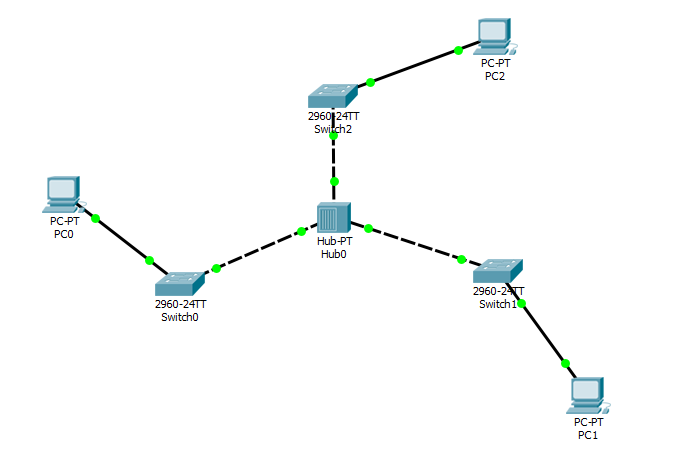
\includegraphics[scale=0.4]{top1.png}
\caption{Topología 1}
\label{fig:top1}
\end{figure}

Luego se nos pide que cada PC envíe datos a otro al mismo tiempo. Notamos que al momento en que los paquetes llegan al HUB colisionan (como se ve en la Figura \ref{fig:topo1}) debido al modo de transmisión que posee dicho dispositivo, es decir, Half Duplex.
\newline Ventajas = Ninguna.
\newline Desventajas = Ineficiente puesto que únicamente funcionaría si sólo una terminal transmite datos.

\begin{figure}[h!]
\centering
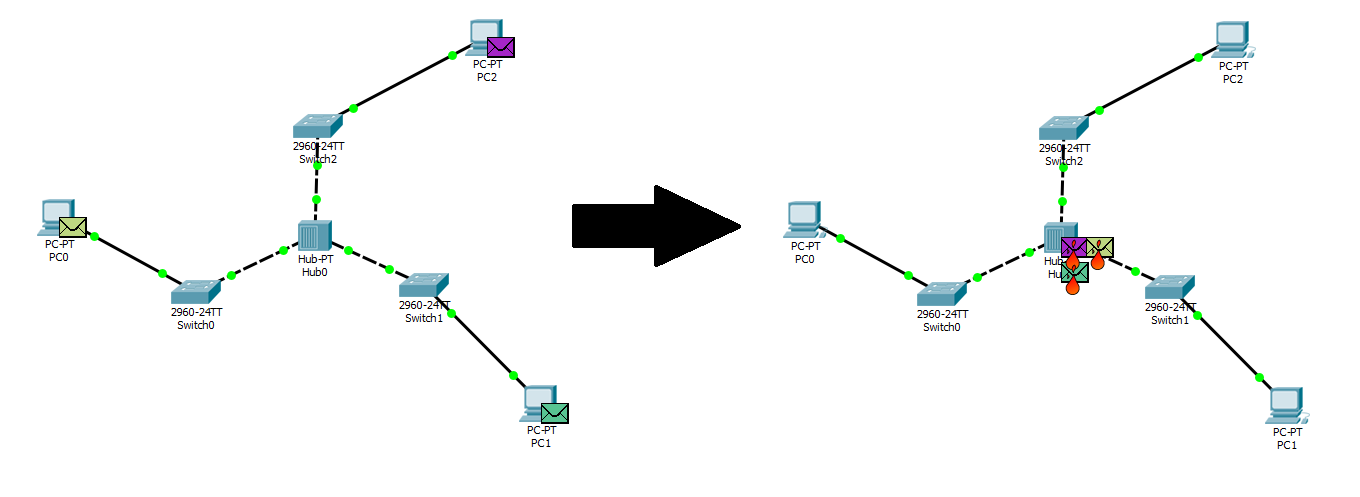
\includegraphics[scale=0.3]{top1,2.png}
\caption{Topología 1 - Envío}
\label{fig:topo1}
\end{figure}

\newpage
En la segunda topología modelada tenemos cuatro HUBs conectados entre sí pero solo a dos de los tres posibles, y cada uno de ellos posee una conexión con un PC como esta representado en la Figura \ref{fig:top2}.

\begin{figure}[h!]
\centering
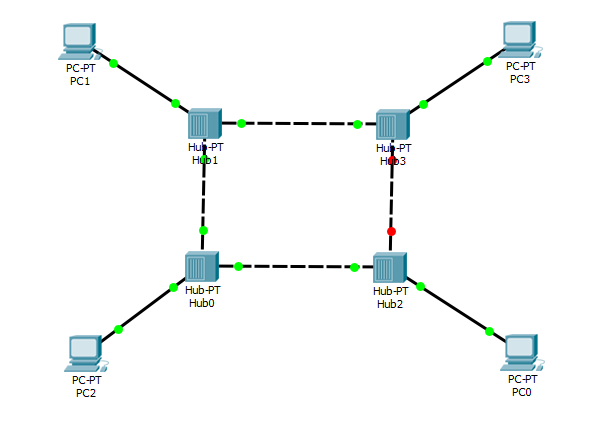
\includegraphics[scale=0.4]{top2.png}
\caption{Topología 2}
\label{fig:top2}
\end{figure}

Se le pide al PC 1 que le envíe un mensaje al PC 0 tal como lo muestra la Figura \ref{fig:topo2} y la transmisión ocurre sin ningún problema.

\begin{figure}[h!]
\centering
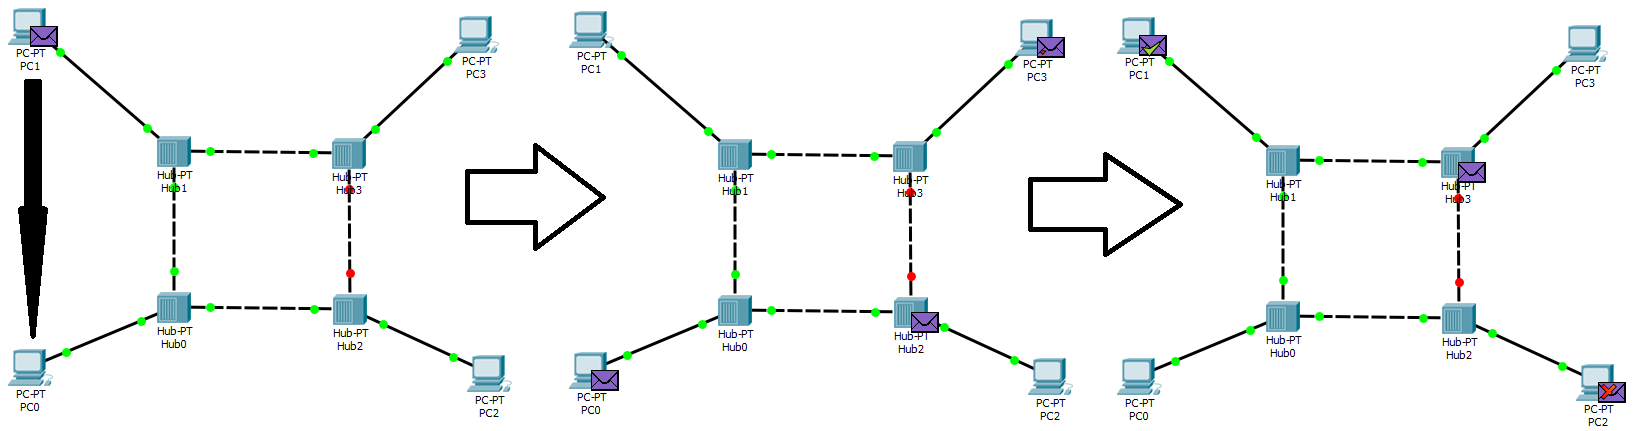
\includegraphics[scale=0.3]{top2,1.png}
\caption{Topología 2 - Envío 1}
\label{fig:topo2}
\end{figure}

Luego se nos pide que el dos PC's transmitan al mismo tiempo ocasionando colisiones y una posterior falla en el envío de datos como se ve en la Figura \ref{fig:topopo2}.
\newline Ventajas = Ninguna
\newline Desventajas = Al igual que la topología anterior, sólo para cuando transmite un PC funciona y, para ese caso, se puede mejorar la topología minimizando los costos, por lo tanto es una topología ineficiente.

\begin{figure}[h!]
\centering
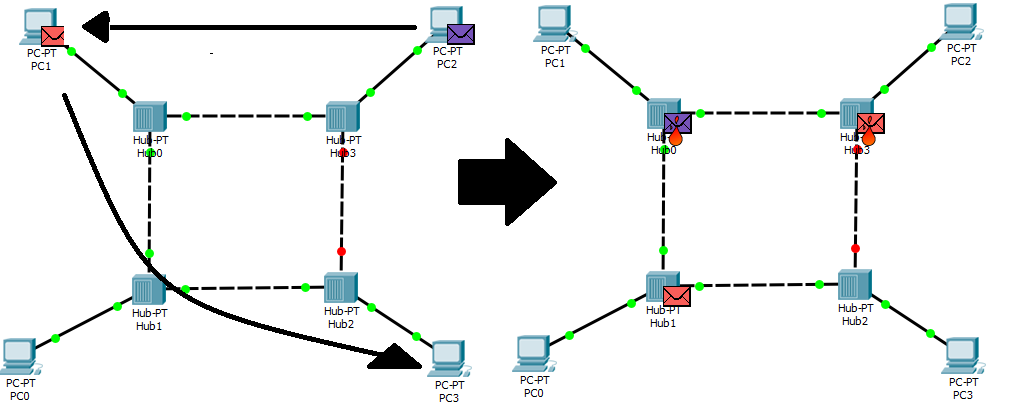
\includegraphics[scale=0.25]{top2,2,1.png}
\caption{Topología 2 - Envío 2}
\label{fig:topopo2}
\end{figure}

\newpage
La tercera y última topología presenta la misma estructura que la anterior, con la diferencia de que, en vez de poseer HUB's, esta tiene Switch's como se ve en la Figura \ref{fig:top3}.

\begin{figure}[h!]
\centering
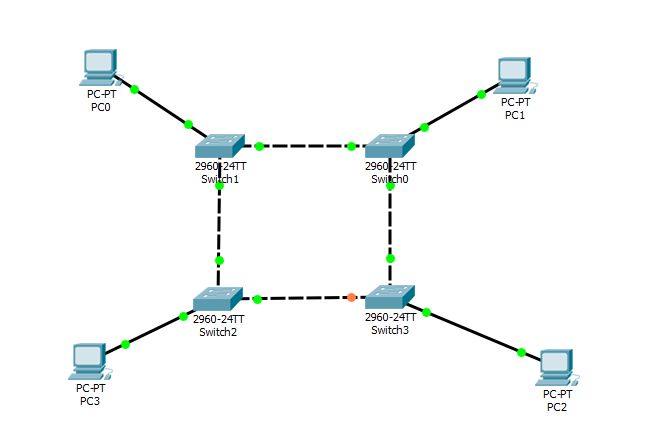
\includegraphics[scale=0.3]{top3.png}
\caption{Topología 3}
\label{fig:top3}
\end{figure}

Se solicita que cada PC envíe datos hacia otro. Notamos que no hay problema con la transmisión de datos puesto que el switch es un dispositivo Full Duplex. (Ver Figura \ref{fig:topo3})
\newline Ventajas = Funciona y la baja probabilidad de colisiones.
\newline Desventajas = Costos.

\begin{figure}[h!]
\centering
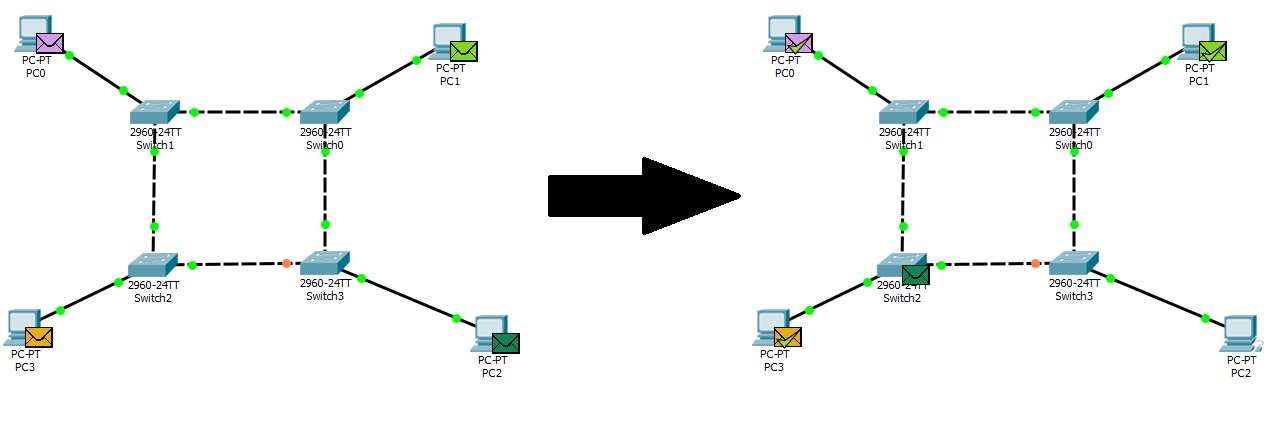
\includegraphics[scale=0.4]{top3,1.png}
\caption{Topología 3 - Envío}
\label{fig:topo3}
\end{figure}

\newpage
\subsection{Actividad 2 \vspace{0.3cm}}
Se nos pide modelar la red del laboratorio de Informática representado en la Figura \ref{fig:Infor} y nos damos cuenta que la principal desventaja de dicha red es el dispositivo central, es decir, el switch, ya que si este falla la red también lo hará.

\begin{figure}[h!]
\centering
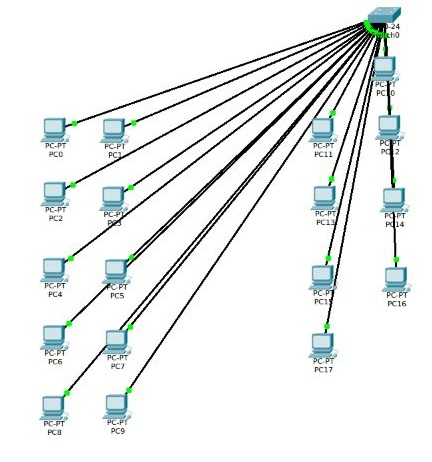
\includegraphics[scale=0.4]{Informatica.jpg}
\caption{Laboratorio de Informática}
\label{fig:Infor}
\end{figure}

Se investigó también sobre los dispositivos conectados en el laboratorio de Telemática, la que esta conformada por 12 PC's Hp Prodesk 400 g2.5 conectados a los switch 4500 de 26 port.
\newpage
\subsection{Preguntas \vspace{0.3cm}}
\begin{enumerate}
    \item ¿Cuáles son los diferentes equipos (con el nombre de los modelos) conectados en la red del laboratorio?\\
    \newline Los equipos conectados a la red del laboratorio de informática son 18 PC's Hp prodesk 400 g2.5 y un switch Catalyst2960.
    
    \item ¿Cuáles son las posibles ventajas y desventajas de las siguientes topologías? (Bus, estrella, malla, malla completa, anillo, árbol).

    \begin{itemize}
    \item Bus:
	\newline Ventajas:
	\newline 	Requiere menos cableado, lo que implica costos menores.
	\newline 	La falla de alguno de sus nodos no afecta a los demás.
	\newline Desventajas:
	\newline 	Diagnostico de falla y aislación complicadas lo que \newline implica una mantención difícil.
	\newline 	La falla del cable central implica la falla de la red.\\
\item Estrella:
	\newline Ventajas:
	\newline 	Fácil instalación y mantención.
	\newline 	El fallo de una de las conexiones con los nodos no afecta a las demás terminales.
	\newline Desventajas:
	\newline 	La falla del dispositivo central significa la falla de la red.\\
\item Malla y Malla completa:
	\newline Ventajas:
	\newline 	Distintas vías para el mismo destino.
	\newline 	La falla de alguna de las conexiones no afecta en nada a la red.
	\newline Desventajas:
	\newline 	Altamente costosas.\\
\item Anillo:
	\newline Ventajas:
	\newline 	Fácil despliegue.
	\newline 	No existen colisiones.
	\newline Desventajas:
	\newline 	Problemas para expandir la red.
	\newline 	Si falla algún conexión o algún nodo, se cae la red.\\
	\newpage
\item Árbol:
	\newline Ventajas:
	\newline 	permite crear un orden jerarquico.
	\newline 	la falla de algun nodo no interrumpe las comunicaciones.
	\newline Desventajas:
	\newline 	Se requiere mucho cableado, lo que implica costos más altos.
	\newline 	La falla del dispositivo principal significa la falla de la red.
    \end{itemize}
    
    \item¿Cuál es la diferencia entre dominio Broadcast y dominio de Colisión?\\
    \newline El dominio de colisión es un segmento de red que comparte el ancho de banda disponible entre múltiples dispositivos terminales; como consecuencia cuando dos o más dispositivos conectados al mismo segmento intentan comunicarse entre sí es posible que se produzca una colisión mientras que el dominio de broadcast es el área lógica en una red de computadoras en la que cualquier computadora conectada a la red puede transmitir directamente a cualquier otra computadora en el dominio sin precisar ningún dispositivo de encaminamiento, dado que comparten la misma subred, dirección de puerta de enlace y están en la misma red de área local.
    \item¿En que facilitaría trabajar a nivel profesional con Packet Tracer? Argumente de manera completa.\\
    \newline Packet Tracer es un programa de simulación de redes que permite experimentar con el comportamiento de red, esto facilita el trabajo a nivel profesional ya que permite comprobar y revisar si la red funcionará de manera esperada además de crear la topología física de la red.
Un ejemplo pude ser el instaurar una red en una oficina, con Packet Tracer puedes idear diferentes formas de colocar esta red y ver si realmente funcionaria como se espera la topología lógica de aquella red.

    \item Dar un ejemplo de en el cual la topología lógica sea diferente a la topología física y argumentar el por qué es así.\\
    \newline La topología Estrella-Anillo, en esta los equipos están conectados a un componente central al igual que en una red en estrella. Sin embargo, estos componentes están enlazados para formar una red en anillo resolviendo el problema de que si un equipo falla afecte al resto de la red. Utilizando el Tokken Passing cada equipo de la topología en estrella-anillo tiene las mismas oportunidades de comunicación y esto permite un mayor tráfico de red entre segmentos.

\end{enumerate}


\newpage
\section{Conclusión \vspace{0.5cm}}
Como resultado de este laboratorio queremos destacar la importancia de conocer las topologías y los dispositivos de red que se usan en ellas puesto que, ya en el ámbito profesional, las buenas decisiones con respecto a este tema van a ser fundamentales, ya sea para reducir costos o para mejorar la fluidez de las redes a implementar.

\end{document}
